
\textbf{Autor: Arbnor, Torben} \\
{ Diese Sicht beschreibt das System auf einer hohen 
  Abstraktionsebene, d.\,h. mit sehr starkem Bezug zur 
  Anwendungsdomäne und den geforderten Produktfunktionen und 
  "~attributen. Sie legt die Grobstruktur fest, ohne gleich in die 
  Details von spezifischen Technologien abzugleiten. Sie wird in den 
  nachfolgenden Sichten konkretisiert und verfeinert. Die 
  konzeptionelle Sicht wird mit {UML}-Komponentendiagrammen 
  visualisiert.
  
  Für die konzeptionelle Sicht haben wir nur den Server modelliert, da die Client-Implementierung bereits 
  über den spezifischen Webbrowser vorliegt, und wir lediglich die Kommunikation zwischen unserem Server und dem
  Webbrowser ermöglichen müssen. 
  Zunächst erläutern wir die einzelnen Komponenten und ihre Verbindung und Aufgaben zueinander, anschließend ist die
  visuelle Darstellung der konzeptionellen Sicht am Ende des Kapitels zu entnehmen.
  
}

\subsection{Server}

{Der Server verfügt über folgende Komponenten:
\begin{itemize}
	\item Model ( in Common)
	\item View
	\item Controller
	\item BusinessLogic
	\item Persistence
	\item Util ( in Common)
	\item Exception ( in Common)
\end{itemize}

{Wir sind bei der Entwicklung der konzeptionellen Sicht hauptsächlich nach dem Model-View-Controller Entwurfsmuster
gegangen und haben
diese um die Komponente BusinessLogic, Util und Exception erweitert.}

\begin{figure}[ht]
	\centering
  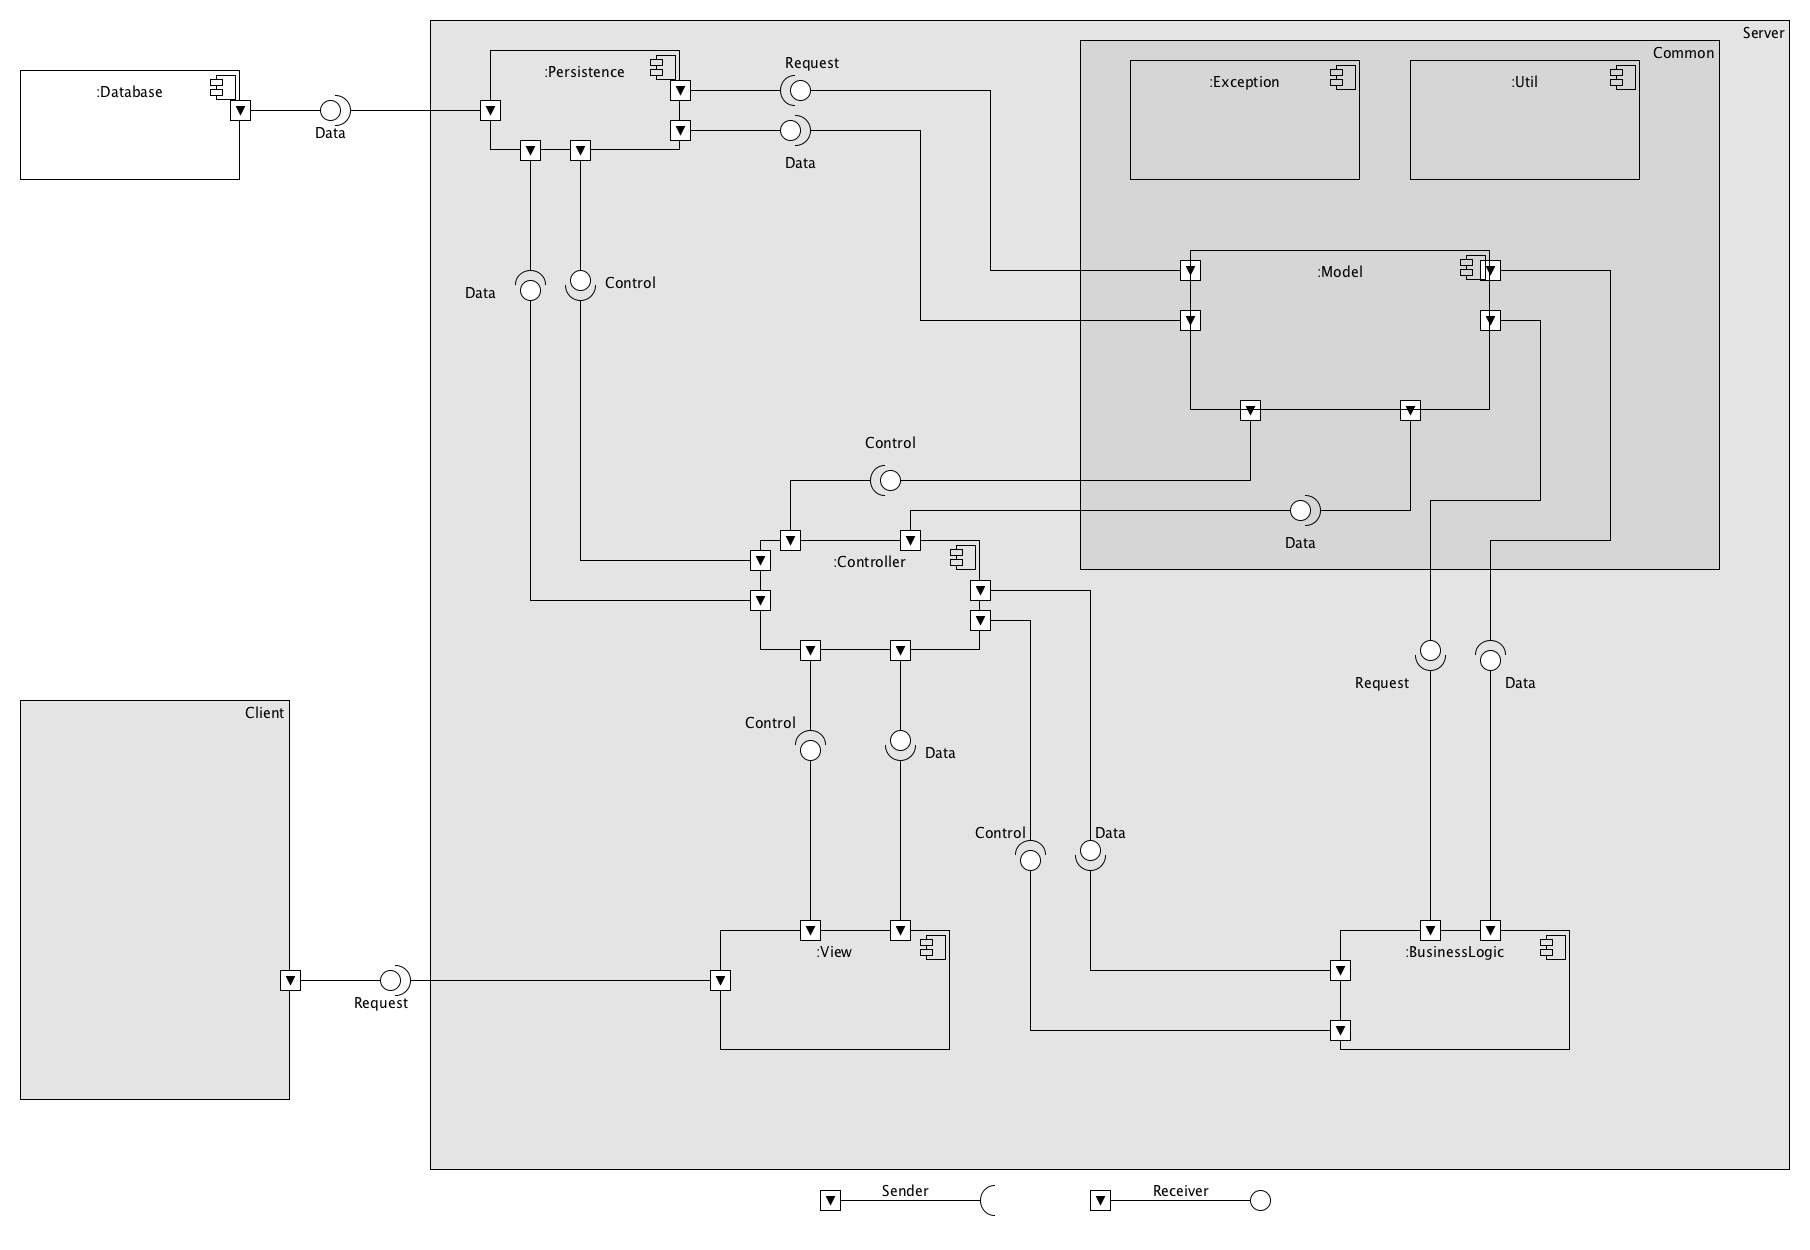
\includegraphics[width=\textwidth,height=15cm,keepaspectratio]{../UMLDiagramme/KonzeptionelleSicht}
	\caption{Konzeptionelle Sicht - Komponentendiagramm}
	\label{fig1}
\end{figure}

\subsubsection{Persistence}
{Die Komponente Persistence ist die Schnittstelle zur Datenbank. An dieser Stelle werden die Datenstrukturen persistiert und Zugriffe auf die Datenbank geregelt. Über View gelangt die Anfrage weiter auf den Controller, welcher 
wiederum auf Persistence zugreift, um Dateninformationen zu erhalten oder zu manipulieren. Dabei hat Persistence  eine direkte Verbindung zum Model in Common, da von dieser Komponente die benötigten Datenstrukturen kommen.}

\subsubsection{View}
{Mit der Komponente View verarbeiten wir die Anfragen, die über die Grafischen Benutzeroberfläche des Clients vom Anwender ausgelöst werden.
Zudem wird über View die Darstellung der Daten geregelt. Dafür erhält View die spezifischen Daten wie z.B die Note
eines Studenten über den Controller, welcher die Daten von dem Model in Common bekommt. View hat nur eine direkte Verbindung zum Controller und zum Client.}
\subsubsection{Controller}
{Der Controller ist die zentrale Verwaltungsschnittstelle zwischen allen Komponenten im Server. Der Controller bekommt von der View eine Benutzeraktion und leitet diese an andere Komponenten, wie BusinessLogic, Common oder der Persistence weiter und gibt der View eine neue Darstellung der Daten zurück.}
\subsubsection{BusinessLogic}
{Die Komponente BusinessLogic  enthält Klassen, die Aufgabe der Geschäftslogik übernehmen.
Hier werden unter anderem die Verschlüsselung und mathematische Grundfunktionalitäten bereit gestellt, um z.B den Durchschnitt einer Prüfung zu berechnen. Die Komponente kann von dem Controller und dem Model in Common angesprochen werden.
}

\subsubsection{Common}
{ Common enthält die Komponenten Exception, Model und Util. Diese Pakete können von allen Paketen außer View genutzt werden. Diese Komponenten tun wir alle in Common (ins Deutsche übersetzt: üblich, gebräuchlich.. ) rein, da diese Komponenten eben sehr oft und von allen Komponenten aus dem Server verwendet werden, uns es daher sinn macht, diese in einem Paket zu vereinen.
}

\begin{figure}[ht]
	\centering
  \includegraphics[width=\textwidth,height=14cm,keepaspectratio]{../UMLDiagramme/common}
	\caption{Konzeptionelle Sicht - Common}
	\label{fig2}
\end{figure}

\newpage
\subsubsection{Model}
Model enthält alle Datenstrukturen, dessen Objekte in der Datenbank über Persistence abgespeichert werden. Zu diesen Datenstrukturen gehören z.B Noten, Termine, User, etc.. .
BusinessLogic hat direkten Zugriff auf die Model-Komponente, genauso wie die Persistence und der Controller.

\subsubsection{Util}
{Die Komponente Util bietet den allen Komponenten aus dem Server Hilfsmethoden an, wie z.B. Assertion, mit dem man unter anderem überprüfen kann ob übergebene Parameter auf Methoden gültig sind oder nicht. Diese Komponente kann von allen anderen Komponenten aus dem Server genutzt werden.
}

\subsubsection{Exception}
{Die Komponente Exception bietet den anderen Komponenten spezifische Exceptions an. Die Komponente kann von allen Komponenten aus dem Server genutzt werden. 
}

\subsection{Einfluss der Strategien auf die konzeptionelle Sicht}
{In diesem Kapitel nennen wir alle Strategien (\ref{K5}), die für die Entwicklung der konzeptionellen Sicht auf das System beigetragen haben und erläutern diese kurz. 
\vspace*{10px}

\textbf{S1: Systemaufbau-MVC}\\
Im vom uns genutzten Prototypen liegt eine Implementierung des Model-View-Controller Entwurfsmuster bereits vor. Daher benutzen wir die Komponenten Model, View und Controller. 
\vspace*{10px}

\textbf{S6: Systemaufbau-Modularisierung}\\
Die Modularisierung ist uns besonders wichtig gewesen, um die Arbeit effizient aufzuteilen.
Für eine bessere Moudlarisierung haben wir die Komponenten Util, BusinessLogic und Exception erstellt. 
\vspace*{10px}

\textbf{S10: Benutzung auf mobilen Geräten}\\
Wir implementieren keinen eigenen mobile-Client, weil wir bisher keine Erfahrung mit der Entwicklung von Smartphone Apps gesammelt haben. Stattdessen gehen wir für den mobilen Client mit einem "responsive-Design" vor, bei den wir lediglich die Resolution der mobilen Endgeräten unter Verwendung des Webbrowser berücksichtigen müssen. Daher ist der Client in allen Fällen ein Browser.
\vspace*{10px}

\textbf{S12: Das Anbinden der Datenbank}\\
Wir haben uns dazu entschieden, die Datenbank über eine Schnittstelle anzubinden. Dadurch ist ein Austausch der Datenbank in der Zukunft ohne größere Probleme machtbar. Dieser Austausch könnte durch geänderte oder neue Anforderungen notwendig werden. Die Datenbankschnittstelle ist in der Komponente Persistence gebündelt. }
\vspace*{10px}

\textbf{S26: Aktualisierung der Inhalte}\\
Das Softwaresystem unterstützt keine Live-Updates. Das Softwaresystem sendet keine Requests an den Client. Das Softwaresystem verarbeitet nur Requests vom Client. Die Datenbank sendet keine Requests an das Softwaresystem. Die Datenbank verarbeitet nur Requests vom Softwaresystem.}